%\begin{tcolorbox}
%Teilt eure Klassendiagramme bitte auf und baut \textbf{kein} einzelnes riesiges Diagramm.
%Getter und Setter Methoden müssen hier nicht modelliert werden.
%Sie sollten aber der klassischen Namenskonvention folgen, um die Nutzung in Sequenzdiagrammen zu ermöglichen.
%\\\\
%Auf jedes Diagramm folgt eine Tabelle, in der die Aufgabe \textbf{jeder} Klasse beschrieben wird.
%\end{tcolorbox}

\section{WebServer}

\begin{figure}[h]
	\centering
	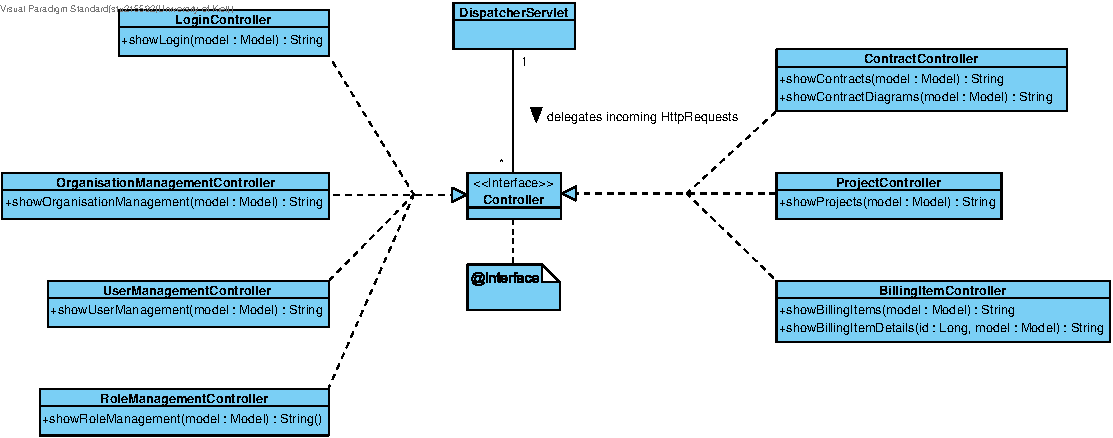
\includegraphics[width=\linewidth]{img/diagrams/Frontend Classes.pdf}
	\caption{Klassendiagramm - Frontend Web}
	\label{fig:klassendiagramm-web}
\end{figure}

\clearpage

\noindent
Klassen, deren Name mit ''Controller'' aufhört, verarbeiten HTTP Requests zu bestimmten Pfaden.
Die zu verarbeitenden Pfade sind pro Gebiet in einem jeweiligen Controller gruppiert.
In der folgenden Tabelle werden für Controller unter ''Aufgabe'' die zu verarbeitenden Pfade sowie die Bedeutung der dazugehörigen Seite aufgeführt.
Die Identifikationsnummern oID (Organisation), diaID (Diagramm), pID (Projekt), cID (Vertrag) und bID (Leistungsposition) sind in manche Pfade direkt integriert. \\

\centering
\begin{longtable}[h]{p{5.3cm} p{8.7cm}}
	\caption{Klassenbeschreibung - Frontend Web}
	\label{table:klassenbeschreibung-web}
	\endlastfoot
	\multicolumn{2}{r}{{Weitergeführt auf der folgenden Seite}} \\
	\endfoot
	\endhead
	\rowcolor[HTML]{C0C0C0} 
	\textbf{Klassenname} & \textbf{Aufgabe} \\
    
	DispatcherServlet & Teil des Spring Frameworks, leitet die HTTP Requests an den jeweils zuständigen Controller weiter \\
	
	\rowcolor[HTML]{E7E7E7} 
	LoginController & /login $\rightarrow$ Login-Seite \\
	
	OrganisationManagementController & /organisation\_overview $\rightarrow$ Management von Organisationen und deren OrgAdmins \\
	
	\rowcolor[HTML]{E7E7E7} 
	UserManagementController & /organisation/\{oID\}/user\_management $\rightarrow$ Management der WebUser einer Organisation \newline\newline
	/organisation/\{oID\}/user\_management/user\_new $\rightarrow$ Hinzufügen eines WebUsers zu einer Organisation \newline\newline
	/organisation/\{oID\}/user\_management/user/\{uID\}/user\_edit $\rightarrow$ Bearbeiten eines WebUsers einer Organisation \\
	
	RoleManagementController & /organisation/\{oID\}/role\_management $\rightarrow$ Management der Rollen einer Organisation \newline\newline
	/organisation/\{oID\}/role\_management/role\_new $\rightarrow$ Hinzufügen einer Rolle zu einer Organisation \newline\newline
	/organisation/\{oID\}/role\_management/role/\{rID\}/role\_edit $\rightarrow$ Bearbeiten einer Rolle einer Organisation \\
	
	\rowcolor[HTML]{E7E7E7} 
	ProjectController & /project\_overview $\rightarrow$ Zeigt alle Projekte an, für welche der WebUser die nötigen Berechtigungen hat \newline\newline
	/project/\{pID\}/show $\rightarrow$ Zeigt die Verträge des Projekts an, für welche der WebUser die nötigen Berechtigungen hat \\
	
	ContractController & /contract\_overview $\rightarrow$ Zeigt alle Verträge an, für welche der WebUser die nötigen Berechtigungen hat \newline\newline
	/project/\{pID\}/contract/\{cID\}/show $\rightarrow$ Zeigt die Leistungspositionen des Vertrags an, für welche der WebUser die nötigen Berechtigungen hat \\
	
	\rowcolor[HTML]{E7E7E7} 
	BillingItemController & /billing\_item\_overview $\rightarrow$ Zeigt alle Leistungspositionen an, für welche der WebUser die nötigen Berechtigungen hat \newline\newline
	/project/\{pID\}/contract/\{cID\}/billing\_item/\{bID\}/show $\rightarrow$ Zeigt Details zur Leistungsposition an \\
	
	DiagramController & /project\_diagram\_overview $\rightarrow$ Zeigt alle Diagramme zu Projekten an, für welche der WebUser die nötigen Berechtigungen hat \newline\newline
	/contract\_diagram\_overview $\rightarrow$ Zeigt alle Diagramme zu Verträgen an, für welche der WebUser die nötigen Berechtigungen hat
\end{longtable}

\clearpage

\section{App}

\section{Backend}
